\begin{figure}[t]
    \centering
    \begin{minipage}{0.245\linewidth}\centering
        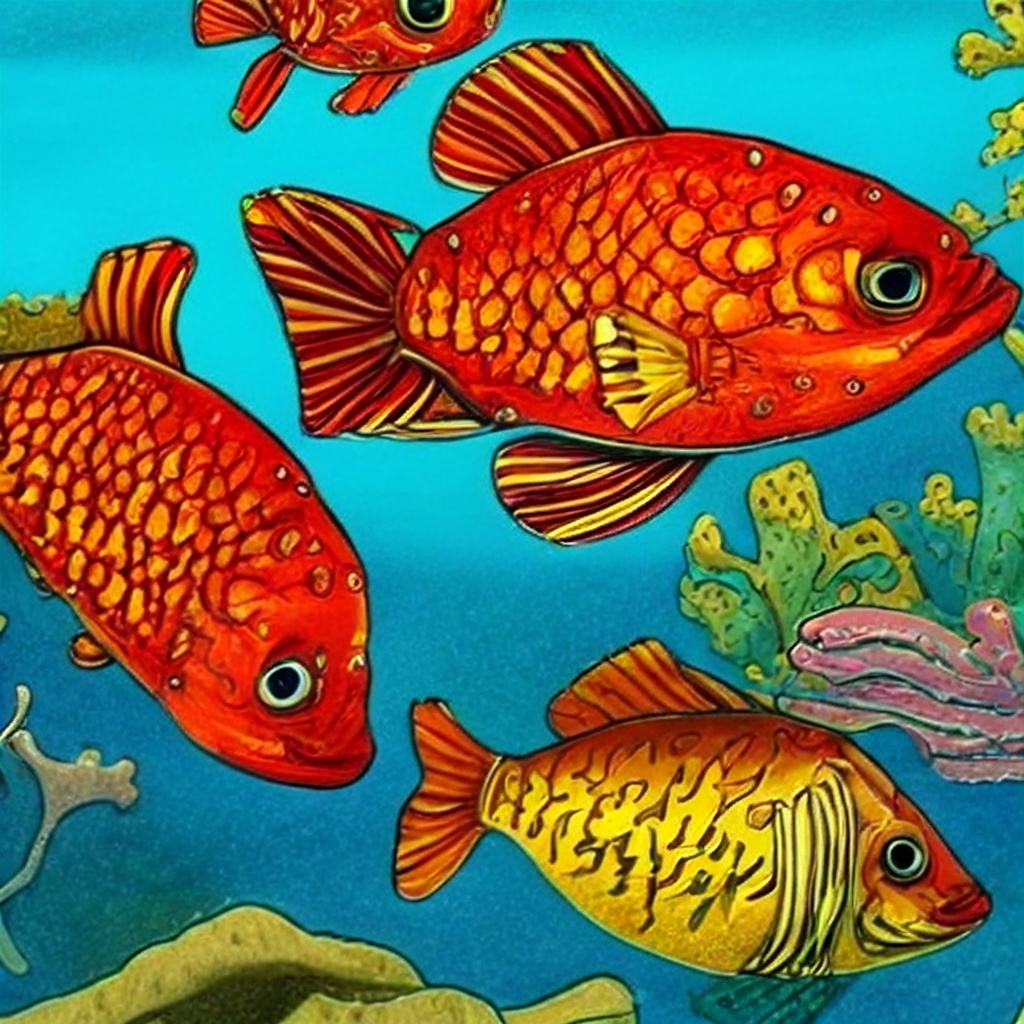
\includegraphics[width=\linewidth]{imgs/blend_source.jpg}\\{\footnotesize source}
    \end{minipage}\hfill
    \begin{minipage}{0.245\linewidth}\centering
        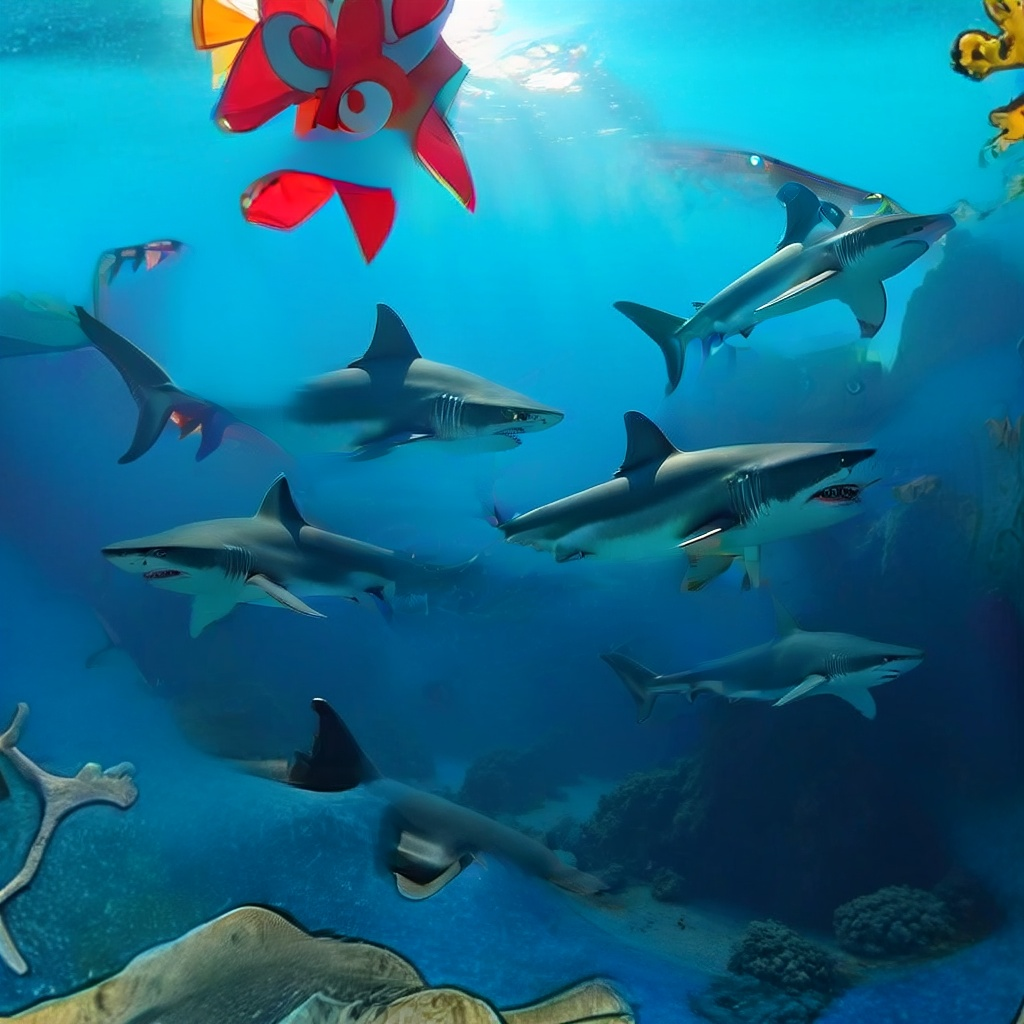
\includegraphics[width=\linewidth]{imgs/blend_baseline.jpg}\\{\footnotesize hard composition}
    \end{minipage}\hfill
    \begin{minipage}{0.245\linewidth}\centering
        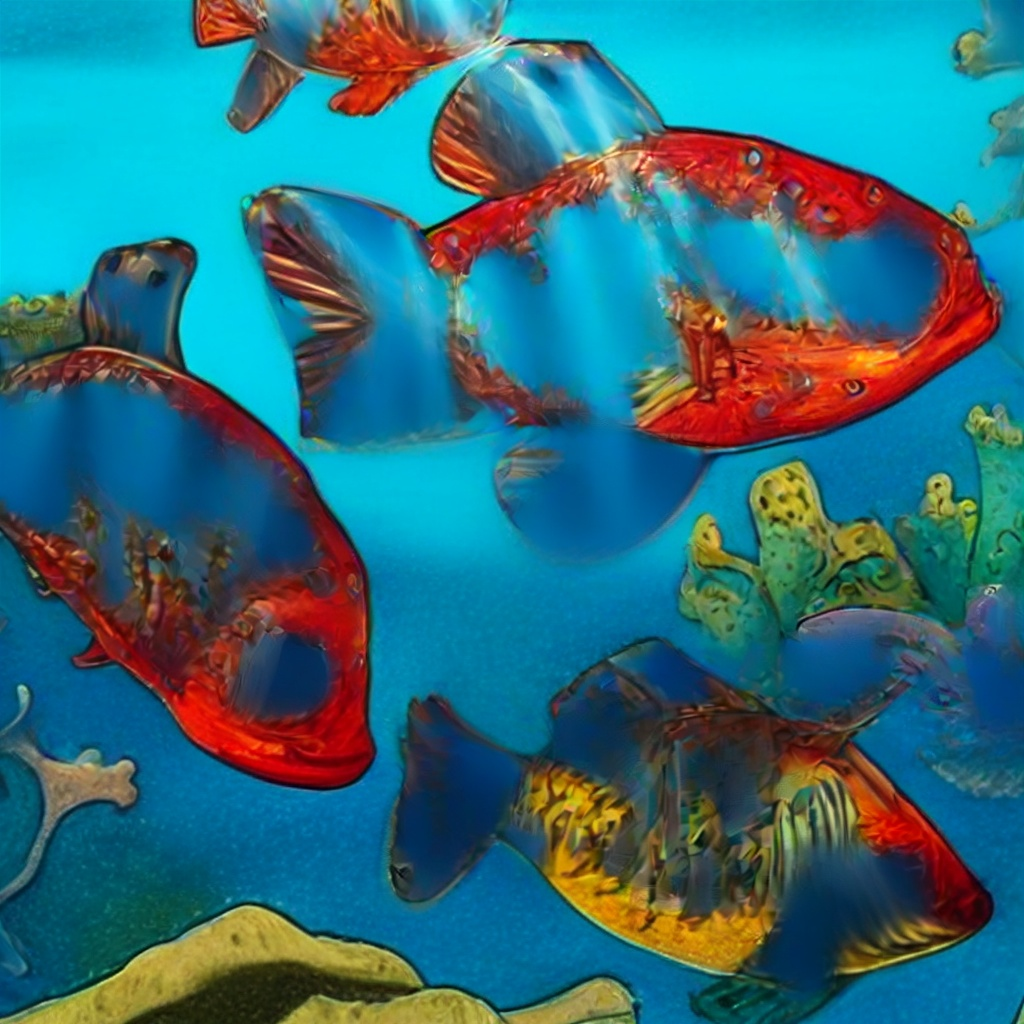
\includegraphics[width=\linewidth]{imgs/blend_hard.jpg}\\{\footnotesize blend, raw mask}
    \end{minipage}\hfill
    \begin{minipage}{0.245\linewidth}\centering
        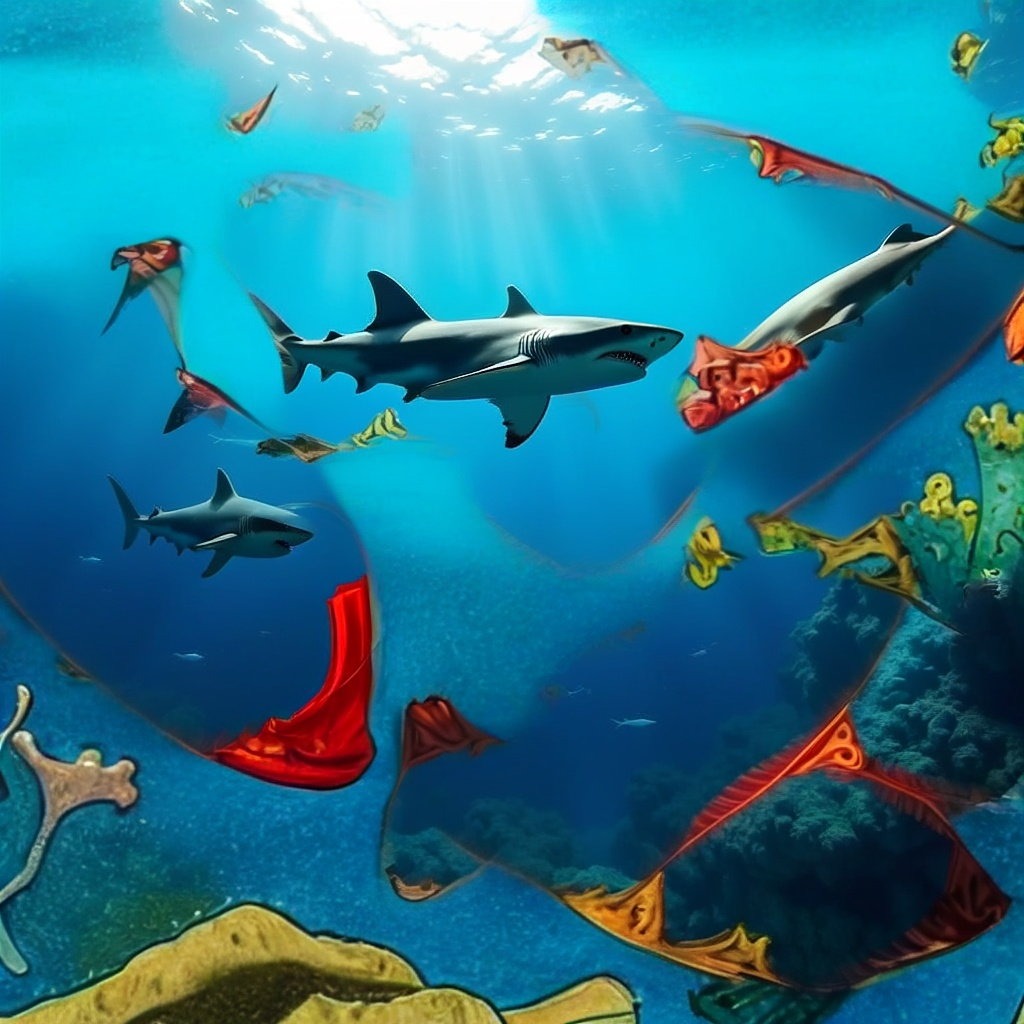
\includegraphics[width=\linewidth]{imgs/blend_best.jpg}\\{\footnotesize blend, cleaned mask}
    \end{minipage}
    \caption{Hard composition versus continuous blending (fish $\to$ shark). Hard composition executes the edit but drifts in style and loses much of the coral background. Blending the continuous residual at full resolution preserves both, but the last-scale attention mask is high-frequency and fragmented, so applying it directly leaves fragments of the source inside the edited region (third panel); a morphological closing and opening of the mask, a soft transition band and coarse anchoring recover the edit (fourth panel). Neither end of this axis dominates: see Sec.~\ref{sec:limitations}.}
    \label{fig:blend}
\end{figure}
